\section{Linearizability}
\label{Sec-Linearizability}
 
Our design provides a linearizable priority queue algorithm. Some operations have multiple possible linearization points by design, requiring careful analysis and implementation.

\textbf{Skiplist.} A successful \texttt{SL::addPar($v$)} (respectively, \texttt{SL::addSeq($v$)}) usually linearizes when it inserts the element in the bottom level of the skip list with a \texttt{CAS} (respectively, with a store), or when the bucket for key $v$ has its counter incremented with a \texttt{CAS} (respectively, with a store). However, a thread inserting a minimal bucket, whenever $v < \mathtt{minValue}$, is required to update \texttt{minValue}. When the sequential part is not empty, only the server can update \texttt{minValue} (without synchronization). When the sequential part is empty, a parallel add with minimal value needs to update \texttt{minValue}.
The adding thread loops until a \texttt{CAS} decreasing \texttt{minValue} succeeds or another thread inserts a bucket with key smaller than $v$. Note that no head-moving operation is taking place (the \texttt{SL::addPar()} threads hold the \texttt{lock}). Threads that succeed changing \texttt{minValue} linearize their operation at the point of the successful \texttt{CAS}. 

The head-moving operations \texttt{SL::moveHead()} and \texttt{SL::chopHead()} execute while holding the \texttt{lock} for writing, which effectively linearizes the operation at the \texttt{lock.release()} instant because: (1) no \texttt{SL::addPar()} is running; (2) no \texttt{SL::addSeq()} or \texttt{SL::removeSeq()} are running, as the server thread is the single thread performing those operations. Head-moving operations do not change \texttt{minValue}, in fact they preclude any changes to it. During these operations, however, threads may still perform elimination, which we discuss next.

\textbf{Elimination.} A unique stamp is used in each request posted in the array entries to avoid the ``ABA'' problem. %This is due to the requirement that only \texttt{add()} values smaller than or equal to the priority queue minimum can eliminate.
Each elimination slot is a 64-bit value that contains 32 bits for the posted value (for \texttt{PQ::add()}) or a special opcode (for \texttt{PQ::removeMin()}) and 32 bits for the unique stamp. In our implementation, the unique stamp is obtained by combining the thread id with the number of operations performed by each thread. %If overflow can become an issue, a different way of generating a unique identifier can be used.
Each thread, either adding or removing, that finds the inverse operation in the elimination array must verify that the exchanged value is smaller than \texttt{minValue}. If so, the thread can \texttt{CAS} the elimination slot, exchanging arguments with the waiting thread. It is possible that the priority queue minimum value is changed by a concurrent \texttt{PQ::add()}. In that case, the linearization point for both threads engaged in  elimination is at the point where the value was observed to be smaller than the priority queue minimum. See Fig.~\ref{fig:correctness_elim}.

\begin{figure}
  \centering
  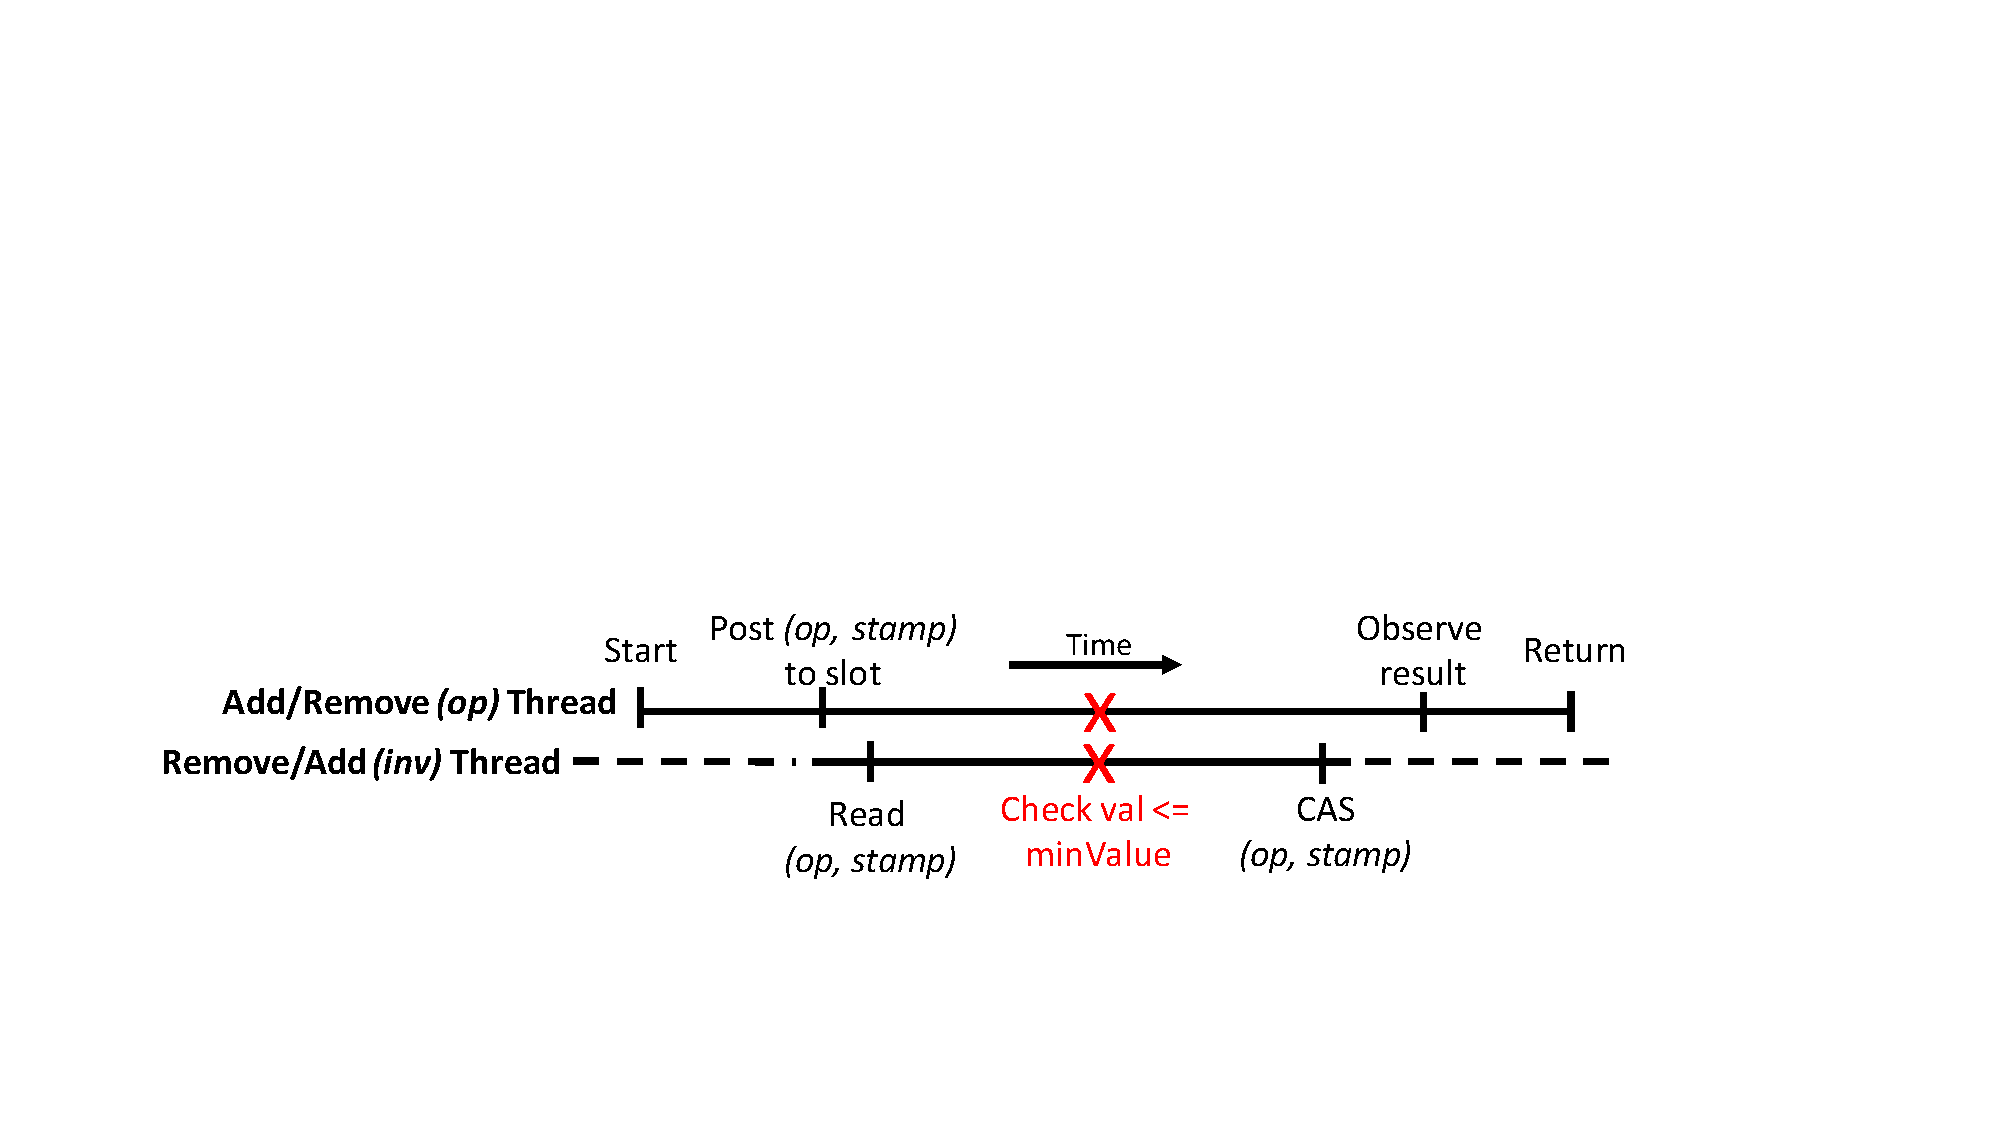
\includegraphics[width=0.9\textwidth]{img/correctness2.pdf}
\caption{Concurrent execution of an \emph{op} thread posting its request to an empty slot, and an \emph{inv} thread, executing a matching operation. The operation by the \emph{inv} thread could begin anytime before the \emph{Read} and finish any time after the \emph{CAS}. The linearization point is marked with a red X.}
\label{fig:correctness_elim}
\end{figure}

The thread performing the \texttt{CAS} first reads the stamp of the thread that posted the request in the array and verifies that it is allowed to eliminate. Only then it performs a \texttt{CAS} on both the value and the stamp, guaranteeing that the thread waiting did not change in the meantime. Because both threads were running at the time of the verification, they can be linearized at that point. Without the unique stamp, the eliminating thread could perform a \texttt{CAS} on an identical request (i.e., identical operation and value) posted in the array by a different thread. The \texttt{CAS} would incorrectly succeed, but the operations would not be linearizable because the new thread was not executing while the suitable minimum was observed.%At the time of the CAS, the minimum could be different, thus elimination should not succeed.

The linearizability of the combining operation results from the linearizability of the skiplist. The threads post their operation in the elimination array and wait for the server to process it. The server first marks the operation as \emph{in progress} by \texttt{CAS}ing INPROG into the slot. Then it performs the sequential operation on the skiplist and writes the results back in the slot, releasing the waiting thread. The waiting thread observes the new value and returns it. The linearization point of the operation happens during the sequential operation on the skiplist, as discussed above. See Fig.~\ref{fig:correctness_server}.

\begin{figure}[htb]
  \centering
  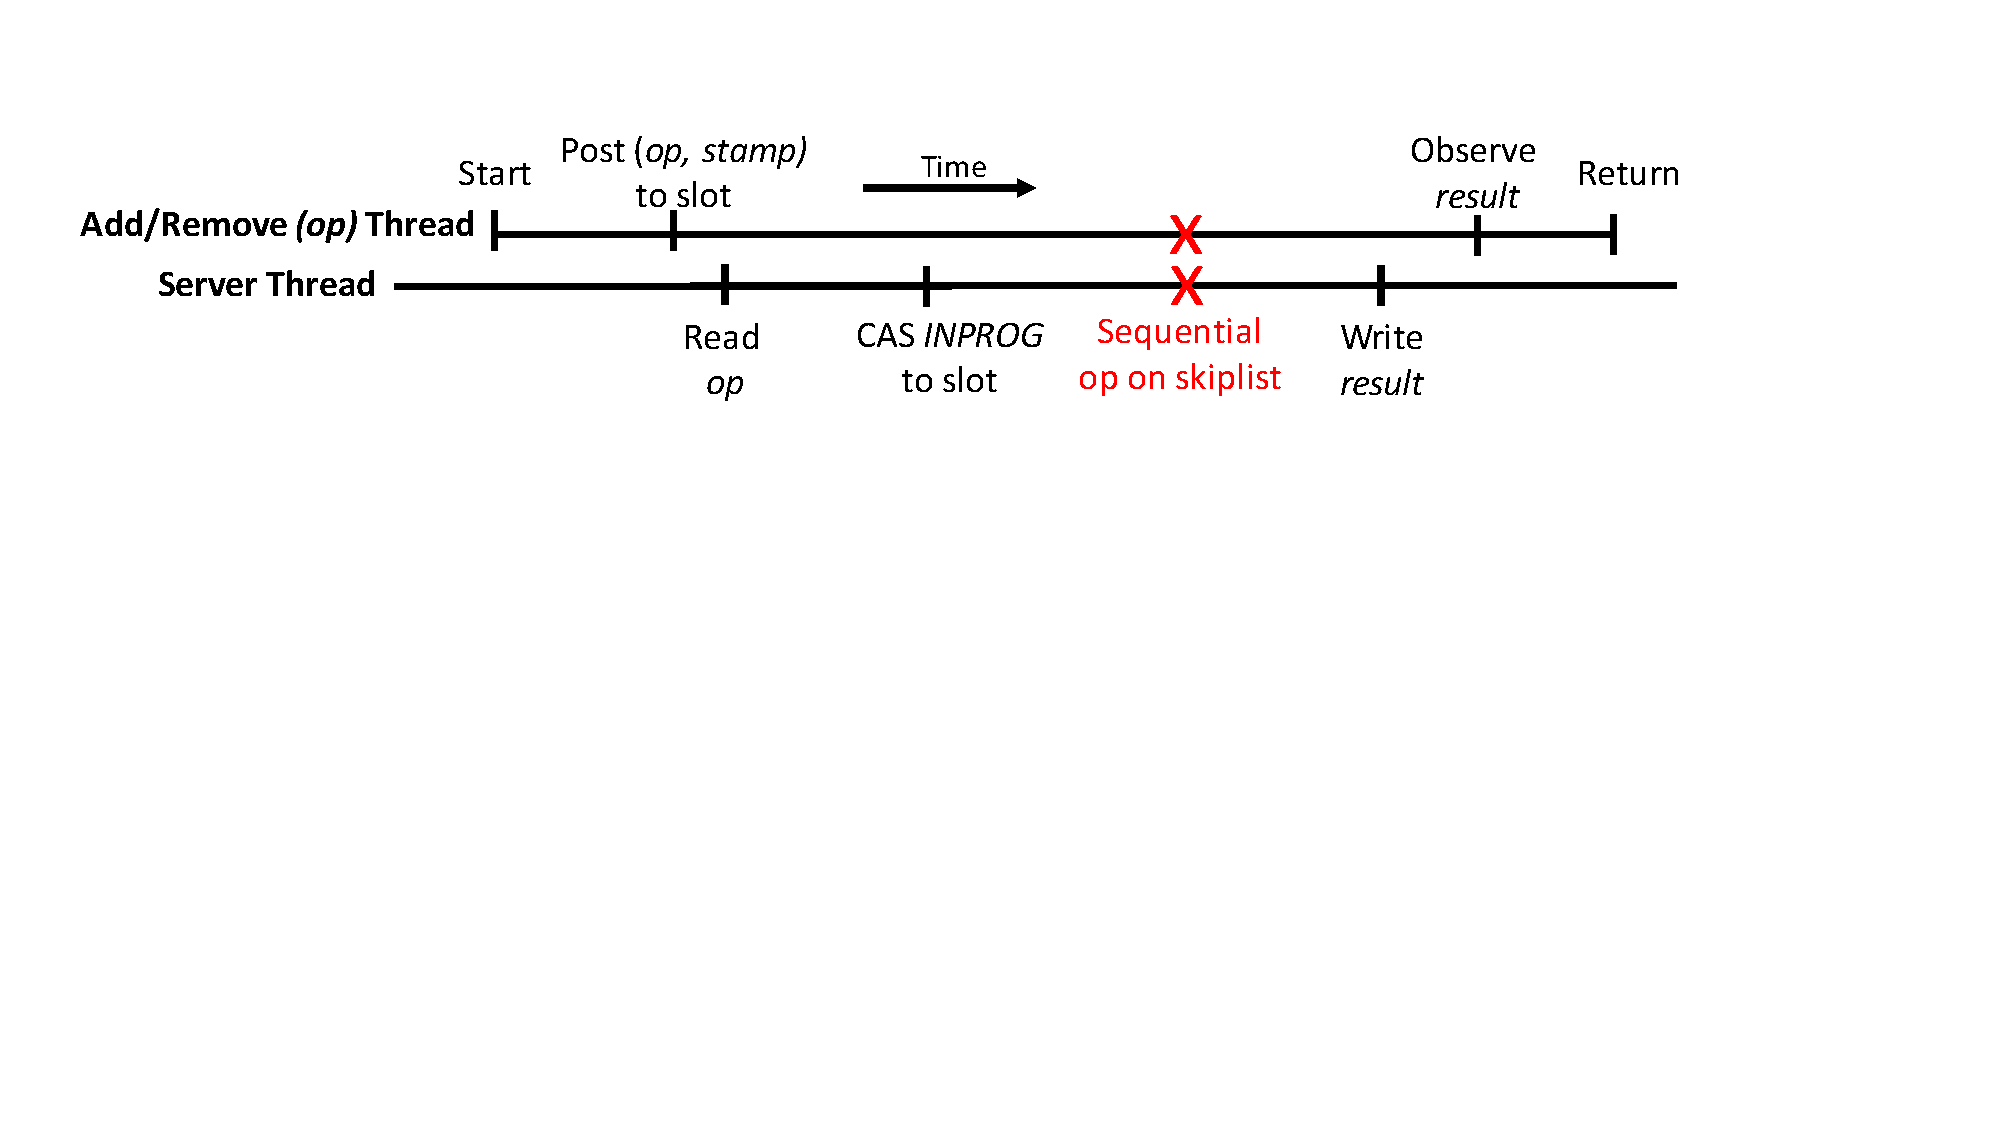
\includegraphics[width=0.9\textwidth]{img/correctness1.pdf}
\caption{Concurrent execution of a client thread and the server thread. The client posts its operation \emph{op} to an empty slot and waits for the server to collect the operation and execute it sequentially on the skiplist. The linearization point occurs in the sequential operation and is marked with a red X.}
\label{fig:correctness_server}
\end{figure}
